\documentclass[submit]{harvardml}

\course{CS181-S22}
\assignment{Assignment \#3}
\duedate{11:59pm EST, March 11, 2022}

\usepackage[OT1]{fontenc}
\usepackage[colorlinks,citecolor=blue,urlcolor=blue]{hyperref}
\usepackage[pdftex]{graphicx}
\usepackage{subfig}
\usepackage{fullpage}
\usepackage{amsmath}
\usepackage{amssymb}
\usepackage{color}
\usepackage{soul}
\usepackage{todonotes}
\usepackage{listings}
\usepackage{common}
\usepackage{enumitem}
\usepackage{bm}
\newcommand{\B}{\text{B}}
\newcommand{\Beta}{\text{Beta}}
\usepackage{pythonhighlight}
\usepackage[mmddyyyy,hhmmss]{datetime}


\setlength\parindent{0em}

\definecolor{verbgray}{gray}{0.9}

\lstnewenvironment{csv}{%
  \lstset{backgroundcolor=\color{verbgray},
  frame=single,
  framerule=0pt,
  basicstyle=\ttfamily,
  columns=fullflexible}}{}

\begin{document}

\begin{center}
{\Large Homework 3: Bayesian Methods and Neural Networks}\\
\end{center}

% FDV: Update for resources, accuracy of submit information **especially any colab components**
% FDV: Make sure to emphasize any plots must be in the pdf submission, we will not be checking code / source 
\subsection*{Introduction}

This homework is about Bayesian methods and Neural Networks.  Section 2.9 in the textbook as well as reviewing MLE and MAP will be useful for Q1. Chapter 4 in the textbook will be useful for Q2.

Please type your solutions after the corresponding problems using this
\LaTeX\ template, and start each problem on a new page.

Please submit the \textbf{writeup PDF to the Gradescope assignment `HW3'}. Remember to assign pages for each question.  \textbf{All plots you submit must be included in your writeup PDF.  }We will not be checking your code / source files except in special circumstances. 

Please submit your \textbf{\LaTeX file and code files to the Gradescope assignment `HW3 - Supplemental'}. 

% FDV: Last year, we pointed folks to
% https://www.cs.ubc.ca/~murphyk/Papers/bayesGauss.pdf
% and folks ended up basically copying from it and not doing any derivation
% For this year, I modified to ask folks to do the full derivation in
% 1.1 but then give them the formula for the marginal likelihood so
% they don't have to derive that.  Open to other variations:
% basically, I think it's probably okay for one part to have a longer
% derivation, but if folks think it's too much, we could have students
% refer to the paper above again or just give them the formula for 1.1
% and ask them to simply interpret it.

\newpage


\begin{problem}[Bayesian Methods]

  This question helps to build your understanding of making
  predictions with a maximum-likelihood estimation (MLE), a maximum a
  posterior estimator (MAP), and a full posterior predictive.

  Consider a one-dimensional random variable $x = \mu + \epsilon$,
  where it is known that $\epsilon \sim N(0,\sigma^2)$.  Suppose we
  have a prior $\mu \sim N(0,\tau^2)$ on the mean. You observe iid data $\{x_i\}_{i=1}^n$ (denote the data as $D$).


\textbf{We derive the distribution of $x|D$ for you.}

\textbf{The full posterior predictive is computed using:}

$$p(x|D)=\int p(x, \mu|D) d\mu =\int p(x|\mu)p(\mu|D) d\mu $$


\textbf{One can show that, in this case, the full posterior predictive distribution has a nice analytic
  form:}
   \begin{align}
        x|D \sim \mathcal{N}\Bigg(\frac{\sum_{x_i\in D}x_i}{n+\frac{\sigma^2}{\tau^2}}, (\frac{n}{\sigma^2}+\frac{1}{\tau^2})^{-1} + \sigma^2\Bigg)
     \end{align}

\begin{enumerate}

  \item Derive the distribution of $\mu|D$.

  \item 
  In many problems, it is often difficult to
  calculate the full posterior because we need to marginalize out the parameters as above (here,
  the parameter is $\mu$). We can mitigate this problem by plugging in
  a point estimate of $\mu^*$ rather than a distribution.

  a) Derive the MLE
  estimate $\mu_{MLE}$.
  % using $p(D|\mu)$.
  
  b) Derive the MAP estimate $\mu_{MAP}$. % using $p(\mu|D)$

  c) What is the relation between $\mu_{MAP}$ and the mean of $x|D$?

  d) For a fixed value of $\mu=\mu^*$, what is the distribution of $x|\mu^*$? Thus, what is the distribution of $x|\mu_{MLE}$ and $x|\mu_{MAP}$?

  e) Is the variance of $x|D$ greater or smaller than the variance of $x|\mu_{MLE}$? What is the limit of the variance of $x|D$ as $n$ tends to infinity? Explain why this is intuitive.


\item Let us compare $\mu_{MLE}$  and $\mu_{MAP}$. There are three cases to consider:

 a) Assume $\sum_{x_i \in D} x_i=0$. What are the values of $\mu_{MLE}$ and $\mu_{MAP}$?

 b) Assume $\sum_{x_i \in D} x_i>0$. Is $\mu_{MLE}$ greater than $\mu_{MAP}$?

 c) Assume $\sum_{x_i \in D} x_i<0$. Is $\mu_{MLE}$ greater than $\mu_{MAP}$?
  
    
\item Compute:

$$\lim_{n \rightarrow \infty} \frac{\mu_{MAP}}{\mu_{MLE}}$$

  \end{enumerate}

  \end{problem}

\newpage
\subsection*{Solution:}

\begin{enumerate}

\item 
Using Bayes' rule, we have

$$p(\mu|D) \propto p(D|\mu)p(\mu)$$

and as the distribution of $D|\mu$ we have the following:

$$p(D|\mu) = \prod_i p(x_i|\mu) = (2\pi\sigma^2)^{-n/2}\exp\left(-\frac{1}{2\sigma^2} \sum_i (x_i-\mu)^2\right)$$
$$\propto_\mu \exp\left(-\frac{1}{2\sigma^2} \sum_i (x_i-\mu)^2\right) $$
$$ = \exp\left(-\frac{1}{2\sigma^2} \sum_i (x_i^2 - 2x_i\mu + \mu^2)\right) $$
$$ = \exp\left(-\frac{1}{2\sigma^2} \left(\sum_i x_i^2 - 2\mu \sum_i x_i + \sum_i \mu^2\right)\right) $$
$$ \propto_\mu \exp\left(-\frac{1}{2\sigma^2} \left( - 2\mu \sum_i x_i + \sum_i \mu^2\right)\right) $$
$$ = \exp\left(-\frac{n}{2\sigma^2} \left( - 2\mu \bar{x} + \mu^2\right)\right) $$

We also know that the prior for $\mu$ is the following, since $\mu\sim \mathcal{N}(0, \tau^2)$

$$p(\mu) \propto \exp\left(-\frac{1}{2\tau^2}  (\mu-0)^2\right) = \exp\left(-\frac{1}{2\tau^2}  \mu^2\right) $$

Multiplying these two to get $P(\mu|D)$ yields the following

$$p(\mu|D) \propto p(D|\mu)p(\mu) = \exp\left(-\frac{n}{2\sigma^2} \left( - 2\mu \bar{x} + \mu^2\right)\right)  \exp\left(-\frac{1}{2\tau^2}  \mu^2\right)$$
$$ = \exp\left(-\frac{n}{2\sigma^2} \left( - 2\mu \bar{x} + \mu^2\right) - \frac{1}{2\tau^2}  \mu^2\right)$$

The product of two Gaussian is a Gaussian, so we know that the above equation can be 
expressed as one. In order to find what the parameters $\sigma_{new}, \mu_{new}$ are of 
this new distribution, we can deduce from the coefficients of $\mu^2$ and $\mu$ above 
what they are.

$$\exp\left(-\frac{n}{2\sigma^2} \left( - 2\mu \bar{x} + \mu^2\right) - \frac{1}{2\tau^2}  \mu^2\right) \stackrel{\text{def}}{=} \exp\left(-\frac{1}{2\sigma_{new}^2}(\mu^2 - 2\mu\mu_{new} + \mu_{new}^2) \right)$$
First we find $\sigma_{new}^2$:
$$ \implies -\frac{1}{2\sigma_{new}^2} \mu^2  = -\frac{1}{2}\left(\frac{1}{\tau^2}+\frac{n}{\sigma^2}\right) $$
$$ \implies \sigma_{new}^2 = \left(\frac{1}{\tau^2}+\frac{n}{\sigma^2}\right)^{-1} $$
and also $\mu_{new}^2$:
$$ \implies  -\frac{1}{2\sigma_{new}^2} (-2\mu\mu_{new}) = \mu\left(\frac{n\bar{x}}{\sigma^2}\right)$$
$$ \implies  \frac{\mu_{new}}{\sigma_{new}^2} = \frac{n\bar{x}}{\sigma^2}$$
$$ \implies  \mu_{new}= \frac{\frac{n\bar{x}}{\sigma^2}}{\frac{1}{\tau^2}+\frac{n}{\sigma^2}}=\frac{n\tau^2\bar{x}}{\sigma^2+n\tau^2}$$


Giving us our distribution of $\mu|D$:
$$\mu|D\sim\mathcal{N}\left(\frac{n\tau^2\bar{x}}{\sigma^2+n\tau^2}, \left(\frac{1}{\tau^2}+\frac{n}{\sigma^2}\right)^{-1}\right)$$

\item

a) $$\mu_{MLE} = \underset{\mu}{\mathrm{argmax}} \,\,p(D|\mu)$$

We find this value by calculating the derivative w.r.t. $\mu$ of $\ln p(D|\mu)$ and setting it to zero. 
We use the simplification of $p(D|\mu)$ from the previous problem.

$$p(D|\mu) \propto_\mu \exp\left(-\frac{n}{2\sigma^2} \left( - 2\mu \bar{x} + \mu^2\right)\right) $$
$$\ln p(D|\mu) \propto_\mu -\frac{n}{2\sigma^2} \left( - 2\mu \bar{x} + \mu^2\right) $$
$$\frac{\partial}{\partial\mu} \ln p(D|\mu) = \frac{n\bar{x}}{\sigma^2} - \frac{n\mu}{\sigma^2} = 0  $$
$$\implies\mu_{MLE} = \bar{x} $$

b) $$\mu_{MAP} = \underset{\mu}{\mathrm{argmax}} \,\,p(\mu|D) = \underset{\mu}{\mathrm{argmax}} \,\,p(D|\mu)p(\mu)$$
Again, we take the derivative of $\ln p(D|\mu)p(\mu)$ w.r.t. $\mu$ and set it to zero. We use the simplification of $p(D|\mu)p(\mu)$ from the 
previous problem.
$$p(D|\mu)p(\mu) \propto_\mu \exp\left(-\frac{n}{2\sigma^2} \left( - 2\mu \bar{x} + \mu^2\right) - \frac{1}{2\tau^2}  \mu^2\right)$$
$$\ln p(D|\mu)p(\mu) \propto_\mu -\frac{n}{2\sigma^2} \left( - 2\mu \bar{x} + \mu^2\right) - \frac{1}{2\tau^2}  \mu^2$$
$$\frac{\partial}{\partial \mu} \ln p(D|\mu)p(\mu) = \frac{n\bar{x}}{\sigma^2} - \frac{n\mu}{\sigma^2} - \frac{\mu}{\tau^2} = 0$$
$$\implies \frac{n\bar{x}}{\sigma^2} - \frac{n\mu_{MAP}}{\sigma^2} - \frac{\mu_{MAP}}{\tau^2} = 0$$
$$\implies \tau^2n\bar{x} - \tau^2n\mu_{MAP} - \sigma^2\mu_{MAP} = 0$$
$$\implies (\tau^2n + \sigma^2)\mu_{MAP} = \tau^2n\bar{x}$$
$$\implies \mu_{MAP} = \frac{\tau^2n\bar{x}}{\tau^2n + \sigma^2}$$

c) $\mu_{MAP}$ is equal to the mean of $x|D$

d) Since $x = \mu + \epsilon $ and $\epsilon \sim \mathcal{N}(0, \sigma^2)$, given a 
fixed $\mu^*$ then 
$$c|\mu_{MLE} = \mathcal{N}(\mu_{MLE}, \sigma^2)$$ and 
$$c|\mu_{MAP} = \mathcal{N}(\mu_{MAP}, \sigma^2)$$


e) The variance of $x|D$ is greater than the variance of $x|\mu_{MLE}$. The variance of $x|D$ as 
$n$ tends to infinity is $\sigma^2$.

This is intuitive since, as $n\to\infty$, $x|D$ is distributed the same way as 
if $\mu$ was held constant ($\mathcal{N}(\mu^*, \sigma^2)$), since an infinitely large
data set, by the law of large numbers, informs us of what our mean is. This gives us a variance
of $\sigma^2$. When $n$ is finite, we have to account for the variance of our prior
for $\mu$, given that that value is not a given. This increases the variance for each our $x$'s.

\item

We have $\sum_{x_i\in D} x_i = n\bar{x}$

a) If $n\bar{x} = 0$, then $\mu_{MLE} = 0$ and $\mu_{MAP} = 0$.

b) If $n\bar{x} > 0$, then $\mu_{MLE} > \mu_{MAP}$.

c) If $n\bar{x} > 0$, then $\mu_{MLE} < \mu_{MAP}$.

\item

$$\lim_{n \rightarrow \infty} \frac{\mu_{MAP}}{\mu_{MLE}} = $$


\end{enumerate}


\newpage

\begin{problem}[Bayesian Frequentist Reconciliation]
    In this question, we connect the Bayesian version of regression with the frequentist view we have seen in the first week of class by showing how appropriate priors could correspond to regularization penalities in the frequentist world, and how the models can be different.
    
    Suppose we have a $(p+1)$-dimensional labelled dataset $\mathcal{D} = \{(\mathbf{x}_i, y_i)\}_{i=1}^N$. We can assume that $y_i$ is generated by the following random process: $$y_i = \mathbf{w}^\top\mathbf{x}_i + \epsilon_i$$ where all $\epsilon_i \sim \mathcal{N}(0,\sigma^2)$ are iid. Using matrix notation, we denote
    \begin{align*}
      \mathbf{X} &= \begin{bmatrix}\mathbf{x}_1 & \ldots & \mathbf{x}_N\end{bmatrix}^\top \in \mathbb{R}^{N \times p} \\
      \mathbf{y} &= \begin{bmatrix} y_1 & \dots & y_N \end{bmatrix}^\top  \in \mathbb{R}^N \\
      \mathbf{\epsilon} &= \begin{bmatrix} \epsilon_1 & \dots & \epsilon_N \end{bmatrix}^\top \in \mathbb{R}^N.
    \end{align*}
    
    Then we can write have $\mathbf{y} = \mathbf{X}\mathbf{w} + \mathbf{\epsilon}$. Now, we will suppose that $\mathbf{w}$ is random as well as our labels! We choose to impose the Laplacian prior $p(\mathbf{w})=\frac{1}{2\tau}\exp\left(-\frac{\|\mathbf{w}-\mathbf{\mu}\|_1}{\tau}\right)$, where $\|\mathbf{w}\|_1=\sum_{i=1}^p |w_i|$ denotes the $L^1$ norm of $\mathbf{w}$, $\mathbf{\mu}$ the location parameter, and $\tau$ is the scale factor.
    
    \begin{enumerate}
    
        \item Compute the posterior distribution $p(\mathbf{w}|\mathbf{X}, \mathbf{y})$ of $\mathbf{w}$ given the observed data $\mathbf{X}, \mathbf{y}$, up to a normalizing constant. You \textbf{do not} need to simplify the posterior to match a known distribution.
        
        \item Determine the MAP estimate $\mathbf{w}_{\mathrm{MAP}}$ of $\mathbf{w}$. You may leave the answer as the solution to an equation. How does this relate to regularization in the frequentist perspective? How does the scale factor $\tau$ relate to the corresponding regularization parameter $\lambda$? Provide intuition on the connection to regularization, using the prior imposed on $\mathbf{w}$.
        
        \item Based on the previous question, how might we incorporate prior expert knowledge we may have for the problem? For instance, suppose we knew beforehand that $\mathbf{w}$ should be close to some vector $\mathbf{v}$ in value. How might we incorporate this in the model, and explain why this makes sense in both the Bayesian and frequentist viewpoints.
        
        \item As $\tau$ decreases, what happens to the entries of the estimate $\mathbf{w}_{\mathrm{MAP}}$? What happens in the limit as $\tau \to 0$?
        
        \item Consider the point estimate $\mathbf{w}_{\mathrm{mean}}$, the mean of the posterior $\mathbf{w}|\mathbf{X},\mathbf{y}$. Further, assume that the model assumptions are correct. That is, $\mathbf{w}$ is indeed sampled from the posterior provided in subproblem 1, and that $y|\mathbf{x},\mathbf{w}\sim\mathcal{N}(\mathbf{w}^T\mathbf{x},\sigma^2)$. Suppose as well that the data generating processes for $\mathbf{x},\mathbf{w},y$ are all independent (note that $\mathbf{w}$ is random!). Between the models with estimates $\mathbf{w}_{\mathrm{MAP}}$ and $\mathbf{w}_{\mathrm{mean}}$, which model would have a lower expected test MSE, and why? Assume that the data generating distribution for $\mathbf{x}$ has mean zero, and that distinct features are independent and each have variance 1.\footnote{The unit variance assumption simplifies computation, and is also commonly used in practical applications.}
        
    \end{enumerate}
  
  
\end{problem}

\subsection*{Solution:}

This is part of the solution m


\newpage
% FDV: We had a lot of debate about this problem, whether it's useful
% for students to have to derive this by hand or not... if we want
% alternatives, ideas could include
%% (1) demonstrate the fact that there are good solutions near any
% starting point (run restarts from many starts, see that the answers
% have good quality but very different weights)
% (2) do a double-descent with linear regression (using very small N).

\begin{problem}[Neural Net Optimization]

  In this problem, we will take a closer look at how gradients are calculated for backprop with a simple multi-layer perceptron (MLP). The MLP will consist of a first fully connected layer with a sigmoid activation, followed by a one-dimensional, second fully connected layer with a sigmoid activation to get a prediction for a binary classification problem. Assume bias has not been merged. Let:
  \begin{itemize}
      \item $\bold{W}_1$ be the weights of the first layer, $\bold{b}_1$ be the bias of the first layer.
      \item $\bold{W}_2$ be the weights of the second layer, $\bold{b}_2$ be the bias of the second layer.
  \end{itemize}
  
  The described architecture can be written mathematically as: $$\hat{y} = \sigma(\bold{W}_2 \left[\sigma \left(\bold{W}_1 \bold{x} + \bold{b}_1\right)\right] + \bold{b}_2)$$
  
  where $\hat{y}$ is a scalar output of the net when passing in the single datapoint $\bold{x}$ (represented as a column vector), the additions are element-wise additions, and the sigmoid is an element-wise sigmoid.
  
  \begin{enumerate}
      \item Let:
      \begin{itemize}
          \item $N$ be the number of datapoints we have
          \item $M$ be the dimensionality of the data
          \item $H$ be the size of the hidden dimension of the first layer. Here, hidden dimension is used to describe the dimension of the resulting value after going through the layer. Based on the problem description, the hidden dimension of the second layer is 1.
      \end{itemize}
      
      Write out the dimensionality of each of the parameters, and of the intermediate variables:

          \begin{align*}
          \bold{a}_1 &= \bold{W}_1 \bold{x} + \bold{b}_1, 
          &\bold{z}_1 = \sigma(\bold{a}_1) \\
          a_2 &= \bold{W}_2 \bold{z}_1 + \bold{b}_2, 
          &\hat{y} = z_2 = \sigma(a_2)
          \end{align*}
          
      and make sure they work with the mathematical operations described above.
      
    \item  We will derive the gradients for each of the parameters.  The gradients can be used in gradient descent to find weights that improve our model's performance. For this question, assume there is only one datapoint $\bold{x}$, and that our loss is $L = -(y \log (\hat{y}) + (1 - y) \log (1 - \hat{y}))$. For all questions, the chain rule will be useful.
    \begin{enumerate}
        \item Find $\frac{\partial L}{\partial b_2}$. 
        
        \item Find $\frac{\partial L}{\partial W_2^h}$, where $W_2^h$ represents the $h$th element of $\bold{W}_2$.
        
        \item Find $\frac{\partial L}{\partial b_1^h}$, where $b_1^h$ represents the $h$th element of $\bold{b}_1$. (*Hint: Note that only the $h$th element of $\bold{a}_1$ and $\bold{z}_1$ depend on $b_1^h$ - this should help you with how to use the chain rule.)
        
        \item Find $\frac{\partial L}{\partial W_1^{h,m}}$, where  $W_1^{h,m}$ represents the element in row $h$, column $m$ in $\bold{W}_1$.
    
    \end{enumerate}
    \end{enumerate}
    
    \end{problem}

\subsection*{Solution:}



\newpage

\begin{problem}[Modern Deep Learning Tools: PyTorch]
  In this problem, you will learn how to use PyTorch. This machine learning library is massively popular and used heavily throughout industry and research. In \verb|T3_P3.ipynb| you will implement an MLP for image classification from scratch. Copy and paste code solutions below and include a final graph of your training progress. Also submit your completed \verb|T3_P3.ipynb| file.

  {\bfseries You will recieve no points for code not included below.}

  {\bfseries You will recieve no points for code using built-in APIs from the \verb|torch.nn| library.}
  
\end{problem}


\subsection*{Solution:}
Plot:

% 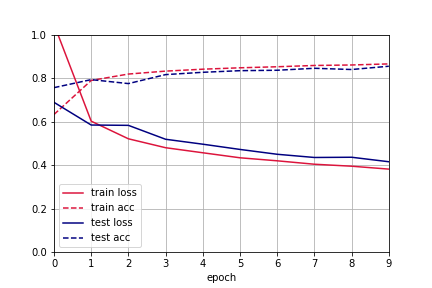
\includegraphics[width=\linewidth]{final_plot}

Code:

\begin{python}
n_inputs = 'not implemented'
n_hiddens = 'not implemented'
n_outputs = 'not implemented'

W1 = 'not implemented'
b1 = 'not implemented'
W2 = 'not implemented'
b2 = 'not implemented'



def relu(x):
    'not implemented'



def softmax(x):
    'not implemented'



def net(X):
  'not implemented'



def cross_entropy(y_hat, y):
  'not implemented'



def sgd(params, lr=0.1):
  'not implemented'



def train(net, params, train_iter, loss_func=cross_entropy, updater=sgd):
  'not implemented'

\end{python}


\newpage
%%%%%%%%%%%%%%%%%%%%%%%%%%%%%%%%%%%%%%%%%%%%%
% Name and Calibration
%%%%%%%%%%%%%%%%%%%%%%%%%%%%%%%%%%%%%%%%%%%%%
\subsection*{Name}

\subsection*{Collaborators and Resources}
Whom did you work with, and did you use any resources beyond cs181-textbook and your notes?

\subsection*{Calibration}
Approximately how long did this homework take you to complete (in hours)? 


\end{document}
